\section{Backgrounds}
\label{sect:bkg}
The backgrounds are studied in two categories, those with 
``misidentified'' \Tau, i.e., events where a quark or gluon jet has been misidentified
as a \Tau, and those with real \Tau decays.
QCD and \wjets events are dominant sources in the first category, while \ttbar, Z+jets, Higgs boson and diboson
events dominate the second category. Background estimates are performed with data-driven methods whenever possible. 
Those backgrounds that are taken from simulation are either validated in dedicated control regions or corrected using data-to-simulation scale factors. The estimates of the main backgrounds are discussed below.

\subsection{\texorpdfstring{QCD background estimation in the $\tauTau$ channel}{QCD background estimation in the tau-tau channel}}
\label{sect:bkgQCD}
Events from QCD multijet production can appear in the signal regions if two hadronic jets are misidentified as a \tauTau pair.
The isolation variable is a powerful discriminant between misidentified and real \Tau candidates. To estimate the QCD multijet contribution, a set of \tauTau control regions (CR) are defined using a less stringent \Tau isolation requirement, referred to hereafter as ``loose'', together with lower thresholds on \mttwo or \SumMT variables. The former is changed from \mttwo $>$ 90\GeV to \mttwo $>$ 40\GeV where the latter is reduced from \SumMT $>$ 250\GeV to \SumMT $>$ 100\GeV. In addition, the requirement on \deltaphi is removed to increase the numbers of events in the control regions. 
%by relaxing the \Tau isolation requirement %(from ``medium'' to ``loose'') 
%and relaxing the \mttwo or \SumMT requirements (from \mttwo $>$ 90\GeV to \mttwo $>$ 40\GeV and from \SumMT $>$ 250\GeV to \SumMT $>$ 100\GeV). 
To reduce contamination from real \tauTau events 
in the control regions with at least one loose \Tau candidate, 
same-sign (SS) \tauTau pairs are selected. Residual contributions from real 
\tauTau and \wjets events (non-QCD events) are subtracted based on Monte Carlo expectations. 
The control regions and signal region are illustrated in Fig.~\ref{fig:ABCDQCD}. 
\begin{figure}[!htb]
\centering
%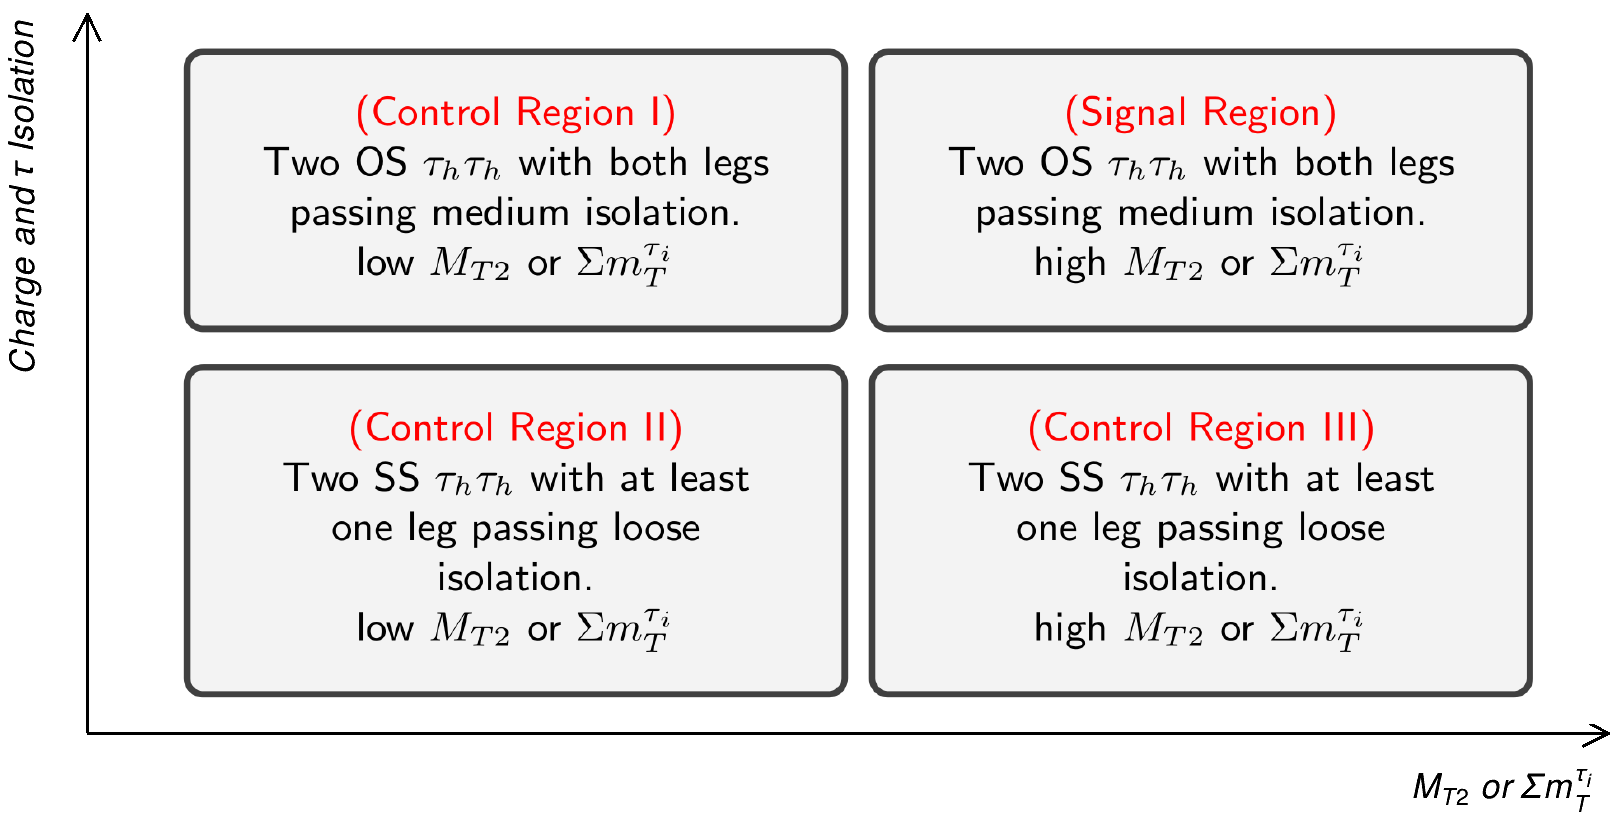
\includegraphics[angle=0,scale=0.28]{Bkg/ABCD.png}
\includegraphics[angle=0,scale=1.15]{Bkg/ABCD.pdf}
\caption{Schematic illustration of four control regions used to estimate the QCD backgrounds. SS and OS stand for same-sign and opposite-sign pairs.}
\label{fig:ABCDQCD}
\end{figure}
In the sample dominated by QCD multijet events (CR1 and CR2), the isolation of misidentified \Tau candidates is verified 
to be almost completely uncorrelated with the search variables (\mttwo or \SumMT).
The QCD background in the signal region is therefore estimated by scaling the number of QCD events with high \mttwo/\SumMT and loosely isolated SS \tauTau (CR3) by a transfer factor, %the ratio of the number of events in CR1 to the number in CR2. 
which is the y-intercept of a horizontal line fitted to the ratio of the number of events in CR1 to the number in CR2 in different bins of the low values of the search variables.
%The QCD background in the signal region is estimated by counting events in the control regions with high \mttwo or \SumMT  
%and loosely isolated SS \tauTau (CR3)
%and scaling by the transfer factor to go from loosely isolated SS to tightly isolated opposite-sign (OS) 
%\tauTau which is evaluated in the low \mttwo or \SumMT regions (CR1 divided by CR2). 
The final estimate of the background 
is corrected by the efficiency of 
the \deltaphi requirement for QCD events. The latter efficiency is measured in CR1 and CR2, 
which are dominated by QCD multijet events. The efficiency is a falling distribution as the function of 
the search variable (\mttwo or \SumMT)
and the value of the closest bin to CR3 ($65<\mttwo<90\GeV$ or $200<\SumMT<250\GeV$) is used conservatively as the 
value of the efficiency in CR3.

The systematic uncertainties on the background estimates include the uncertainty on the validity of the assumption that isolation and \mttwo or \SumMT are not correlated and the uncertainties on the residual 
SM backgrounds which  are subtracted based on Monte Carlo expectations. 
The latter includes both the statistical uncertainty of the simulated 
events and also a 22\% systematic uncertainty that will be discussed in Section~\ref{sect:sys} 
assigned uniformly to all simulated events.

The number of data events in CR3 after subtracting the non-QCD events is 4.81 $\pm$ 2.57 (8.62 $\pm$ 3.55) in \binone (\bintwo).
The transfer factors are measured to be 0.91 $\pm$ 0.12 and 0.89 $\pm$ 0.11 in the low \mttwo and \SumMT, respectively, and 
the correction for the \deltaphi efficiency is 0.03 $\pm$ 0.04 in \binone and 0.15 $\pm$ 0.08 in \bintwo. 
All reported uncertainties are the quadratic sum of the statistical and systematic uncertainties.

 
Table \ref{4QCDbg} 
\begin{table}[!htb]
\begin{center}
\caption{The estimated QCD multijet background event yields in the \tauTau channel. The first two uncertainties are statistical and systematic uncertainties of the method, the last uncertainty is the extra systematic uncertainty due to correlation assumptions.}
\begin{tabular}{|l|c|}
\hline
 Signal Region       & QCD  Estimation\\
\hline\hline
\tauTau \binone      & 0.13 $\pm$ 0.06(stat) $\pm$ 0.18(sys) $\pm$ 0.10(fit) \\
\tauTau \bintwo      & 1.15 $\pm$ 0.39(stat) $\pm$ 0.70(sys) $\pm$ 0.25(fit) \\
\hline
\end{tabular}
\label{4QCDbg}
\end{center}
\end{table}
summarizes the estimation of the QCD background contribution in the two signal regions after extrapolation from 
the control regions and correcting for the \deltaphi efficiency. %The uncertainties due to the statistic of the CR3 is reported 
%as the statistical uncertainty ``stat'' and the other uncertainties are shown as ``sys''. 
To evaluate the uncertainties for the transfer factor and \deltaphi efficiency due to correlation assumptions, 
different fit models are tested. 
%For both transfer factor and \deltaphi efficiency following procedure is used.
%To measure the values in the control region 
Fitting the whole range of the low values of the search variables by a horizontal line or a line with a constant slope 
or using the value of the last bin before entering the signal region are examined. 
The weighted average of the estimates is compared with the reported values 
in Table \ref{4QCDbg} to extract the uncertainty shown as ``fit'' in the table.


\subsection{\texorpdfstring{\wjets background estimation in the $\tauTau$ channel}{W+jets background estimation in the tau-tau channel}}
\label{sect:bkgW}
The contribution of the \wjets background in the \tauTau channels is taken from simulated events. The simulation is validated using a data control sample: 
%In different signal regions after the final requirement of \mttwo $>$ 90\GeV or \SumMT $>$ 250\GeV, 
%the \wjets Monte Carlo has large statistical uncertainties and the predicted value is not reliable. 
%The efficiencies of the final selection requirements, $\epsilon_{\rm M_{T2}}=\frac{N_{\rm M_{T2}>90}}{N_{\rm M_{T2}>40}}$ for  \binone and $\epsilon_{\SumMT}=\frac{N_{\SumMT>250}}{N_{40<\rm M_{T2}<90}}$ for \bintwo, generally referred to as $\epsilon_{FS}$, are evaluated in MC after relaxing some kinematic selections. 
%The final estimations can be read as:
%\begin{equation}
%N_{\rm SR} = N_{\rm Before~Final~Selection} \times \epsilon_{FS}.
%\end{equation}
%where, $N_{\rm Before~Final~Selection}$ is the number of \wjets events just before applying the final selection 
%(\mttwo $>$ 90\GeV for \binone and \SumMT $>$ 250\GeV for \bintwo) and $N_{\rm SR}$ is the final estimation of \wjets events in %the signal region.
\begin{equation}
N_{\rm SR} = N_{\rm Before~Final~Selection} \times \epsilon_{FS}.
\end{equation}
Here $N_{\rm SR}$ is the estimation of \wjets events in the signal region. $N_{\rm Before~Final~Selection}$ is the number of 
\wjets events before applying the final selection (\mttwo $>$ 90\GeV for \binone and \SumMT $>$ 250\GeV for \bintwo), but after applying all other selections, including \mttwo $>$ 40\GeV for \binone and 40 $<\mttwo<$ 90\GeV for \bintwo.  
$\epsilon_{FS}$ is $\epsilon_{ \rm M_{T2}}= \frac{N (\rm M_{T2}>90)}{N (\rm M_{T2}>40)}$ for \binone or  
$\epsilon_{\SumMT}=\frac{N (\SumMT>250)}{N(40<\rm M_{T2}<90)}$ for \bintwo. $N_{\rm Before~Final~Selection}$ is 31.93$\pm$6.40 and 29.13$\pm$6.22 for \binone and
\bintwo, respectively, where the given uncertainties arise from the limited number of simulated events. 


The  efficiency of the final selection ($\epsilon_{FS}$) is evaluated in a \wjets simulated sample with a pair of opposite-sign \Tau where the \Tau candidates 
are selected with the same identification requirements as the signal region, but with looser kinematic selection to improve statistics.
Additional signal selection requirements, such as \deltaphi or lepton veto, are applied one by one such that two orthogonal subsamples (passing and failing) are obtained. The $\epsilon_{FS}$ quantity is calculated in all subsamples. The values are found to be consistent with the value from the relaxed sample 
within the statistical uncertainties. 
%their weighted average is taken as the final estimate for $\epsilon_{FS}$ with weights corresponding to the size of the simulated sample at each step. %The uncertainty on the \Tau energy scale introduces the largest variation on $\epsilon_{FS}$. This variation is considered as a systematic uncertainty on the estimated efficiency.
The measured $\epsilon_{FS}$ from the relaxed samples are  
0.028 $\pm$ 0.010 and 0.098 $\pm$ 0.032 for \binone and \bintwo, respectively.
The uncertainty of the \Tau energy scale is also taken  into account in the uncertainty on $\epsilon_{FS}$.


The \wjets simulated sample is validated in data using a same-sign \muTau control sample, where both the normalization and $\epsilon_{FS}$ are checked. 
The ratio of data and Monte Carlo expectation is found to be 1.05 $\pm$ 0.13 (1.02 $\pm$ 0.09) for \binone(\bintwo) 
which is compatible with unity, within the uncertainties. 
For $\epsilon_{FS}$, 
to take into account the difference between the data and Monte Carlo values, the Monte Carlo prediction in each
of the two signal regions is corrected by the ratio of the two values which is 0.73 $\pm$ 0.57 (1.49 $\pm$ 0.38)
for \binone(\bintwo) and its uncertainty is also taken to be the systematic uncertainty and referred to as ``shape''.

Table \ref{tbl:Wbkg} summarizes the results of  the method for different signal regions of the \tauTau channel.
\begin{table}[!htb]
\begin{center}
\caption{The \wjets estimation results in both search regions. 
The systematic uncertainty ``sys'' comes from the maximum
variation of the estimation found  from varying the \Tau energy scale within its uncertainty. 
The ``shape'' takes into account the difference between the shape of the search variable distribution in data and simulation.}
\begin{tabular}{|l|c|}
\hline
Signal Region & \wjets Estimation\\
\hline
\tauTau \binone & 0.70 $\pm$ 0.21 (stat) $\pm$ 0.09 (sys) $\pm$ 0.54 (shape)\\
\tauTau \bintwo & 4.36 $\pm$ 1.05 (stat) $\pm$ 1.14 (sys) $\pm$ 1.16 (shape)\\
\hline
\end{tabular}
\label{tbl:Wbkg}
\end{center}
\end{table}

\subsection{Drell-Yan background estimation}
The Drell-Yan (DY) background yield is obtained from Monte Carlo simulation. 
The simulated sample includes decay to different lepton pairs ($ee$, $\mu\mu$ and $\tau\tau$). 
The contribution from \Z$\rightarrow \ell \ell$ and \Z$\rightarrow \tau \tau\rightarrow \ell \ell$ events is found to be very small, because the misidentification probability for $\ell\rightarrow$  \Tau 
is significantly low.  
The dominant background events are \Z$\rightarrow \tau \tau\rightarrow \ell \Tau$ and \Z$\rightarrow \tau \tau\rightarrow \Tau \Tau$ decays.
The misidentification probability for  \Tau $\rightarrow\ell$ is also low, so the probability 
to have contribution from \Z$\rightarrow \tau \tau\rightarrow \Tau \Tau$ events in the \leptonTau channels is negligible.
%are for the \leptonTau channels the contribution from these events which have a real lepton 
%and a misidentified \Tau is evaluated in the next section, when \wjets contribution is estimated.
The simulation is validated in a \muTau control region obtained by removing the \deltaphi
requirement and by inverting the \Z boson veto and also by requiring \mttwo $<$ 20\GeV,  40 $<$ \tauMT $<$ 100\GeV.  
The distributions of invariant mass of \muTau system for data and simulated events are in good agreement.
The transverse momentum of the \Z boson system, which is correlated with 
\mttwo, is also well reproduced in simulation. Table \ref{tbl:DYbkg}
\begin{table}[!htb]
\begin{center}
\caption{DY background yield expected in four signal regions. 
%The first uncertainty is statistical and the second is systematic. The systematic uncertainties assigned to the central values are discussed in Section \ref{sect:sys}.}
Only the statistical uncertainties are reported.}
\begin{tabular}{|l|c|}
\hline
Signal Region      &  DY Estimation\\
\hline\hline
\eTau              & 0.19  $\pm$  0.04\\\hline%  $\pm$ 0.05 \\\hline
\muTau             & 0.25  $\pm$  0.06\\\hline%  $\pm$ 0.07 \\\hline
\tauTau \binone    & 0.56  $\pm$  0.07\\\hline%  $\pm$ 0.16 \\\hline
\tauTau \bintwo    & 0.81  $\pm$  0.56\\\hline%  $\pm$ 0.23 \\

\end{tabular}
\label{tbl:DYbkg}
\end{center}
\end{table}
summarizes the DY contribution in different signal regions. 
For \leptonTau channels, only the contributions from the real lepton + \Tau are reported. 
A separate method is developed in Section~\ref{sect:bkgFake} to estimate the misidentified contamination in these channels.

\subsection{\texorpdfstring{Misidentified \Tau in the \leptonTau channels}{Misidentified tau in the lepton-tau channels}}
\label{sect:bkgFake}
%This contribution is estimated using a fake rate method.
This contribution is estimated using a method that takes into account the probability that a loosely isolated misidentified or real \Tau,
passes the tight isolation.
If the signal selection is done using the \Tau candidates which pass the ``loose'' isolation instead of ``tight'', 
the number of loose \Tau candidates ($N_{\rm Loose}$) is:

\begin{equation}
N_{\rm Loose} = N_{\rm Real} + N_{\rm Fake}
\end{equation}
where $N_{\rm Real}$ is the number of real \Tau candidates and $N_{\rm Fake}$ is the number of misidentified 
\Tau candidates. If the selection is tightened, the number of tight \Tau candidates ($N_{\rm Tight}$)  is

\begin{equation}
 N_{\rm Tight} = r_{\rm Real}\times N_{\rm Real} + r_{\rm Fake}\times N_{\rm Fake}
\end{equation} 
where $r_{\rm Real}$ ($r_{\rm Fake}$) is the real (fake) rate, the probability that a loosely selected real (misidentified) \Tau candidate passes the  tight  selection. 
%The loose category ($N_{\rm Loose}$) can be divided to two parts, tight ($N_{\rm Tight}$) and non-tight ($N_{\rm NTight}$), 
One can obtain the following expression by eliminating $N_{\rm Real}$:

\begin{equation}
   N_{\rm Fake}\times (r_{\rm Fake}-r_{\rm Real}) = (N_{\rm Tight} - r_{\rm Real}\times N_{\rm Loose})
\end{equation}
Here $r_{\rm Fake}\times N_{\rm Fake}$ is the contamination of misidentified \Tau candidates to the signal region. 

The fake rate ($r_{\rm Fake}$) is measured as the ratio of tightly selected \Tau candidates to loosely 
selected \Tau candidates in a sample which is dominated by misidentified \Tau candidates. 
This is done in a data sample with same selection as \leptonTau, except a reversed
\MPT requirement, i.e., \MPT $<$ 30\GeV. The fake rate is measured to be 0.54 $\pm$ 0.01.
%A consistent value is measured for the fake rate.  
The real rate ($r_{\rm Real}$) is measured in simulated DY events; it is found to 
be $r_{\rm Real}$ = 0.766 $\pm$ 0.003 and almost independent of \mttwo. 
%For both fake rate and real rate, the evaluated uncertainties are low and a 
A conservative relative systematic uncertainty of 5\% is assigned to the central value of $r_{\rm Real}$ to cover its 
fluctuations for different values of \mttwo.
%, although by varying the selections, no significant change in the values is seen.
To validate the method, it is applied to a \wjets simulated sample  
where the fake rate is evaluated with the same method as used for data. 
The result is close to $r_{\rm Fake}$ = 0.54. To cover the difference, a 5\% relative systematic uncertainty is
assigned to the central values of the fake rates.
The method correctly predicts the number of \leptonTau background events in this sample, within the 
uncertainties.
These include statistical uncertainties due to the number of events in the 
sidebands (loosely selected \Tau) as well as 
systematic uncertainties.
The uncertainties on the %variation of the method to estimate the 
fake rate and the real rate %and their statistical uncertainties 
are negligible compared to the statistical uncertainties associated with 
the sidebands. 

The estimates of the misidentified \Tau contamination in the two \leptonTau 
channels are summarized in Table~\ref{Tab.FakeEstimation}. 
\begin{table}[!htb]
\begin{center}
\caption{Estimation of the misidentified \Tau contribution in the signal region of the \leptonTau channels. The total systematic is the
quadrature sum of the fractional systematics. All uncertainties are relative.
$r_{\rm Fake}$ ($r_{\rm Real}$) is shorthand for fake (real) rate.}
\begin{tabular}{|l|c|c|c|c|c|}
\hline
Channel    & Total Fake & stat &  $r_{\rm Fake}$ sys & $r_{\rm Real}$  sys & Total Unc \\\hline\hline
\muTau     &   8.15     &   56\%    &  18\%    & 5\%   & 59\%  \\
\eTau      &   3.30     &  101\%    &  17\%    & 2\%  & 102\%  \\
\hline
\end{tabular}
\label{Tab.FakeEstimation}
\end{center}
\end{table}
The relative statistic and systematic uncertainties are reported separately. 
Since the fake rate and real rate are in common between the two 
\leptonTau channels, the total systematic uncertainties are considered 
fully correlated between the two channels.
